\documentclass[12pt,a4paper]{article}
\usepackage[UTF8]{ctex}
\usepackage{amsmath,amssymb}
\usepackage{xcolor}
\usepackage{hyperref}
\usepackage{geometry}
\usepackage{graphicx}
\geometry{margin=2.5cm}

\title{Hardware Compilation / 硬件编译}
\author{QuoNic}
\date{}

\begin{document}
\maketitle

\begin{center}
\textbf{Compilation / 编译} | 难度：中级 | 预计时间：15 分钟
\end{center}

\tableofcontents
\newpage

\section{为什么需要？}

硬件编译将量子电路编译为硬件可执行的格式。

\subsection{经典局限}
\begin{itemize}
  \item 量子电路无法直接在硬件上执行
  \item 需要编译为硬件格式
\end{itemize}

\subsection{量子优势}
\begin{itemize}
  \item 硬件编译可以优化量子电路
  \item 适配不同量子硬件
  \item 提高执行效率
\end{itemize}

\subsection{实际应用}
\begin{itemize}
  \item 量子硬件执行
  \item 电路优化
  \item 硬件适配
\end{itemize}

\section{快速上手}

\begin{verbatim}
from quonic.compile import hardware_compile

# 硬件编译
result = hardware_compile(circuit, backend='ibmq_manila')
print(f'Compiled circuit: {result.circuit}')
\end{verbatim}

\textbf{预期输出}：
\begin{verbatim}
Compiled circuit: ...
\end{verbatim}

\section{原理详解}

\subsection{电路图}

\begin{center}
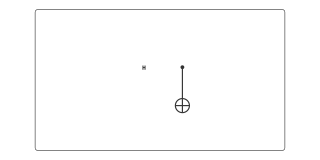
\includegraphics[width=0.6\textwidth]{../../images/hardware_compile_circuit.svg}
\end{center}

\subsection{数学推导}

硬件编译：
\begin{equation}
C_{\text{hardware}} = \text{compile}(C_{\text{logical}}, \text{backend})
\end{equation}

\subsection{几何解释}

硬件编译将逻辑电路映射到物理硬件。包括门分解、电路优化、映射等步骤。

\section{代码详解}

\begin{verbatim}
from quonic.compile import hardware_compile

# hardware_compile(circuit, backend)
# circuit: 量子电路
# backend: 目标后端

result = hardware_compile(
    circuit=circuit,
    backend='ibmq_manila'
)

# result.circuit: 编译后的电路
# result.depth: 电路深度
# result.gate_count: 门数量
print(f'Compiled circuit: {result.circuit}')
\end{verbatim}

\section{进阶用法}

\subsection{场景 1：不同后端}

\begin{verbatim}
from quonic.compile import hardware_compile

# 不同后端
r1 = hardware_compile(circuit, backend='ibmq_manila')
r2 = hardware_compile(circuit, backend='ibmq_quito')
r3 = hardware_compile(circuit, backend='ibmq_belem')
\end{verbatim}

\section{适用场景}

\subsection{量子硬件执行}

硬件编译将量子电路编译为硬件可执行的格式。这是在真实量子硬件上运行电路的必要步骤。

\subsection{电路优化}

硬件编译可以优化量子电路，减少门数量和电路深度。

\section{常见问题}

\subsection{硬件编译和量子编译有什么区别？}

硬件编译是量子编译的一个步骤。量子编译还包括门分解、映射等步骤。

\subsection{硬件编译的性能如何？}

硬件编译的性能取决于后端特性和电路复杂度。

\section{学习路径}

\subsection{前置知识}
\begin{itemize}
  \item 量子电路
  \item 量子硬件
  \item 量子编译
\end{itemize}

\subsection{继续学习}
\begin{itemize}
  \item 量子硬件
  \item 电路优化
  \item 量子执行
\end{itemize}

\section{完整示例代码}

\subsection{示例 1：基本硬件编译}

\begin{verbatim}
from quonic.compile import hardware_compile

result = hardware_compile(circuit, backend='ibmq_manila')
print(f'Compiled circuit: {result.circuit}')
\end{verbatim}

\section{下载}

\begin{itemize}
  \item [hardware\_compile.py](https://github.com/ChrisLee0721/QuoNic/blob/main/examples/hardware_compile/hardware_compile.py)
\end{itemize}

\end{document}
